\documentclass[11pt]{article}

\usepackage[margin=1in]{geometry}
\usepackage[T1]{fontenc}
\usepackage[utf8]{inputenc}
\usepackage{lmodern}
\usepackage{microtype}
\usepackage{graphicx}
\usepackage{booktabs}
\usepackage{array}
\usepackage{longtable}
\usepackage{amsmath, amssymb}
\usepackage{siunitx}
\usepackage{caption}
\usepackage{subcaption}
\usepackage{hyperref}
\usepackage[numbers,sort&compress]{natbib}
\usepackage{enumitem}
\usepackage{xcolor}
\usepackage{listings}
\usepackage{float}
\newcolumntype{P}[1]{>{\raggedright\arraybackslash}p{#1}}

\hypersetup{colorlinks=true, linkcolor=blue!50!black, citecolor=blue!50!black, urlcolor=blue!50!black}
\graphicspath{{figures/}}
\sisetup{round-mode=places, round-precision=3}
\setlist[itemize]{noitemsep, topsep=2pt}
\setlist[enumerate]{noitemsep, topsep=2pt}

\lstset{
  basicstyle=\ttfamily\small,
  breaklines=true,
  frame=single,
  columns=fullflexible
}

\title{From Coda Categories to Temporal Operators: An Unsupervised Reanalysis of Sperm Whale Coda Structure in Annotated Dominica Data and DSWP Audio Recordings}
\author{Computational bioacoustics reanalysis}
\date{June 2026}

\begin{document}
\maketitle

\begin{abstract}
Sperm whale codas are traditionally represented as short sequences of clicks whose inter-click intervals define a coda type. Recent work has shown that this representation is incomplete: rhythm, tempo, rubato, and ornamentation form a combinatorial ``phonetic alphabet'', while newer work suggests additional spectral, vowel-like structure. This paper reanalyzes two public resources: the annotated coda and dialogue artifacts released with \path{pratyushasharma/sw-combinatoriality}, and audio recordings from the Dominica Sperm Whale Project (DSWP) Hugging Face corpus. The analysis does not align individual DSWP audio recordings to individual rows of the annotated dialogue table. Instead, it uses the annotated corpus for within-recording sequential tests, and the DSWP audio recordings for independent acoustic-phonetic tests. We introduce a temporal-operator hypothesis: the first recoverable layer of meaning in these corpora is not a dictionary of object labels, but a set of timed operators that maintain, transfer, intensify, or close a shared social-acoustic state. Empirical support comes from five observations: (i) DSWP audio recordings contain an unsupervised inter-click timing alphabet with six robust gap bands centered near 29, 46, 80, 137, 222, and 362 ms; (ii) dense long recordings are motif-compressed rather than random; (iii) in the annotated dialogue table, the dominant rhythm class R2 behaves as a carrier frame rather than as a simple isolated type; (iv) sparse and dense rhythm classes such as R0 and R17 participate in high-switch and high-overlap transitions, especially R0--R2 and R17--R0; and (v) fine timing features predict speaker switching better than rhythm class alone in grouped cross-validation. These results do not establish literal translations. They justify a reproducible functional lexicon in which coda forms are glossed as candidate interactional operators such as carrier, handoff, escalation, boundary, and closure.
\end{abstract}

\noindent\textbf{Keywords:} sperm whale codas; bioacoustics; animal communication; temporal grammar; Project CETI; Dominica Sperm Whale Project; unsupervised phonology; operator semantics.

\section{Introduction}

Sperm whales (\textit{Physeter macrocephalus}) produce social vocalizations known as codas: stereotyped groups of broadband clicks with structured inter-click intervals (ICIs). Codas have long been associated with social identity, matrilineal social units, and vocal clans \citep{rendell2003clans,gero2016identity,whitehead2003sperm}. The standard analytical abstraction represents a coda by its click count and ICI pattern. This abstraction has made possible decades of work on coda repertoires, clan dialects, and individual or group identity cues. It also imposes a risk: once a signal is reduced to a named coda type, other dimensions of timing, tempo, density, overlap, stress, and acoustic shape can be treated as noise.

The present study begins from the opposite assumption. A coda is treated as a timed act. Its observable form is the tuple
\begin{equation}
    x_i = (n_i, d_i, \Delta_{i,1:n_i-1}, a_i, r_i, t_i, s_i),
\end{equation}
where $n_i$ is click count, $d_i$ is duration, $\Delta_{i,j}$ are inter-click intervals, $a_i$ denotes acoustic amplitude features when audio is available, $r_i$ denotes a recording or timeline identifier, $t_i$ denotes onset time within that timeline, and $s_i$ denotes an annotated speaker identity when available. The goal is not to assign a fixed English word to $x_i$. The goal is to ask whether the form of $x_i$ changes the likely future of the exchange: who enters next, whether the next signal overlaps, whether the sequence continues, and whether a bout boundary is near.

This paper therefore proposes a conservative functional translation layer. A form has a candidate meaning if it reliably changes an interactional state. In this sense, a signal may be glossed as a \emph{carrier}, \emph{handoff}, \emph{escalation}, or \emph{closure} operator without claiming that the same signal means a specific English sentence. This notion is weaker than semantic translation but stronger than descriptive classification. It is also compatible with the emerging view that sperm whale codas have multiple independently variable dimensions: timing, rhythm, tempo, rubato, ornamentation, and potentially spectral quality.

\section{State of the art}

\subsection{Coda repertoires, clans, and identity}

Classical sperm whale bioacoustics established that codas are socially meaningful and culturally patterned. Vocal clans are defined by distinctive coda repertoires, and clan-specific ``identity codas'' can organize association and cooperation among social units \citep{rendell2003clans,gero2016identity}. These results make it implausible that codas are only incidental by-products of movement or arousal. They also show that a coda type can carry social information without being a lexical word in the human sense.

Prior interactional work also showed that codas occur in coordinated exchanges, including overlapping and matching behavior \citep{schulz2008overlapping}. These observations motivate analyses that treat codas not only as isolated objects but also as events in a multi-whale timeline.

\subsection{The combinatorial timing alphabet}

The major recent shift is the Project CETI analysis of contextual and combinatorial structure \citep{sharma2024contextual}. In that work, codas are decomposed into rhythm, tempo, rubato, and ornamentation. The authors argue that these axes combine to produce a much larger space of distinguishable codas than traditional coda-type labels capture. They also emphasize that codas are produced in exchanges, not merely in isolation, and that context-dependent features such as rubato and ornamentation are sensed and acted upon by whales. The associated GitHub and Zenodo release provides the annotated artifacts reanalyzed here \citep{swcombinatoriality}.

\subsection{Automatic detection and large-scale audio modeling}

Parallel work has addressed the engineering problem of detecting and annotating codas automatically. \citet{gubnitsky2025automatic} present an automatic coda detector and annotator based on graph-based clustering, designed to separate codas from echolocation clicks and to handle overlapping sources. Transformer-based modeling has also entered the field: WhAM is a masked acoustic-token model for synthesizing and analyzing sperm whale codas, trained on coda recordings and evaluated on downstream tasks such as rhythm, social-unit, and spectral-feature classification \citep{paradise2025wham}. The DSWP Hugging Face corpus used here is associated with that modeling program and is described as containing 1,501 sperm whale coda audio files from Dominica, each containing at least one extracted coda \citep{dswpdataset}.

\subsection{Spectral dimensions and coda vowels}

Recent phonological work further expands the space of relevant features. \citet{begus2025vowels} report vowel- and diphthong-like spectral patterns in sperm whale codas, arguing that spectral properties are structured and may add a dimension independent of timing and click count. A subsequent phonological analysis argues that these coda vowels pattern along several dimensions analogous to human phonology \citep{begus2026phonology}. These results support a methodological caution: timing alone is not the full signal. The present paper nevertheless focuses on timing and simple amplitude features because those are the dimensions recoverable from the public artifacts analyzed here.

\subsection{Dialect evolution}

Coda timing also participates in cultural evolution. A 2026 study of Mediterranean sperm whales reports dialect variation in an isolated population, including faster and slower variants of related rhythmic forms across eastern and western basins \citep{hersh2026mediterranean}. This is relevant because it shows that tempo and timing differences can be socially and historically meaningful, not merely acoustic noise.

\section{What is changed here}

This reanalysis changes the unit of interpretation. Instead of beginning with the question, ``What word does this coda mean?'', it begins with the question, ``What operation does this timed form perform on the next state of the exchange?'' Four methodological changes follow.

\begin{enumerate}
    \item \textbf{Separate corpora, separate claims.} The annotated dialogue artifacts are used for sequential and speaker-switch analyses because they contain recording identifiers, onsets, durations, and speaker IDs. The DSWP audio recordings are used for acoustic-phonetic analysis only. No individual DSWP audio recording is asserted to correspond to any individual row of the annotated dialogue table.
    \item \textbf{Rhythm labels are treated as partial summaries.} The release rhythm index $R$ is used, but it is not treated as a complete sign. Continuous duration, normalized ICI geometry, click density, and ornamentation are retained.
    \item \textbf{Meaning is operationalized as change in future distributions.} A coda form is considered functionally meaningful if it changes the distribution of immediate outcomes: next speaker, next gap, overlap, or bout position.
    \item \textbf{Raw audio is used to check what tabular encodings hide.} The audio recordings are analyzed for timing alphabets, dense-train structure, amplitude contour, and stereo-source proxies. These results provide independent constraints on how codas should be represented.
\end{enumerate}

\section{Data}

\subsection{Annotated coda and dialogue artifacts}

The annotated timing data come from the public release associated with \citet{sharma2024contextual} and \path{pratyushasharma/sw-combinatoriality} \citep{swcombinatoriality}. The main sequential table analyzed here is \path{sperm-whale-dialogues.csv}. It contains 3,840 coda rows, 219 distinct recording identifiers (\path{REC}), 11 speaker IDs (\path{Whale}), onset times (\path{TsTo}), durations, click counts, and up to 28 ICI columns. The associated release artifacts \path{rhythms.p}, \path{mean_codas.p}, \path{ornaments.p}, and \path{tempos-dict.p} provide the rhythm, mean-rhythm template, ornament, and tempo information used below. A second table, \path{DominicaCodas.csv}, is used only as a background reference for traditional coda-type labels and clan/unit association; it is not the source of the transition statistics reported here.

\subsection{DSWP audio recordings}

The acoustic analysis uses audio recordings from the Dominica Sperm Whale Project corpus distributed as \path{orrp/DSWP} on Hugging Face \citep{dswpdataset}. The public dataset card describes 1,501 coda audio files, about 45 minutes of audio, recorded off Dominica from 2005 to 2018 using towed hydrophones, portable recorders, and animal-borne tags. The numerical acoustic results in this paper are computed on a decodable local DSWP audio subset for which 1,041 recordings passed the click-detection threshold of at least three detected clicks. These recordings are treated as isolated snippets: they provide acoustic structure but no behavioral context, no speaker identity, no row-level mapping to the annotated dialogue table, and no reliable temporal order across files.

\begin{table}[H]
\centering
\caption{Data roles. The distinction is central: sequential claims are derived only from the annotated dialogue table, while acoustic-phonetic claims are derived only from DSWP audio recordings.}
\label{tab:data_roles}
\begin{tabular}{P{0.25\linewidth}P{0.29\linewidth}P{0.34\linewidth}}
\toprule
Resource & Fields or features used & Claims supported \\
\midrule
Dialogue table with rhythm and ornament artifacts & REC, Whale, onset, duration, click count, ICIs, rhythm index $R$, ornament flag $O$ & Within-recording adjacency, speaker switching, overlap, bout position, microtiming effects, AUC prediction of next-speaker switch \\
\addlinespace
Reference coda table & traditional coda labels, clan/unit/individual metadata & Background interpretation of labeled repertoires; not used for transition or AUC statistics \\
\addlinespace
DSWP audio recordings & detected clicks, ICIs, amplitude contour, stereo delay when available & Timing alphabet, density families, motif compression, acoustic dimensions hidden by tabular labels \\
\bottomrule
\end{tabular}
\end{table}

\section{Notation and definitions}

\subsection{Coda representation}

For coda $i$, let $n_i$ be the number of clicks, $d_i$ its duration, and
\begin{equation}
    \Delta_i = (\Delta_{i,1}, \ldots, \Delta_{i,n_i-1})
\end{equation}
be its inter-click interval vector. The normalized interval vector is
\begin{equation}
    p_i = \frac{\Delta_i}{\sum_{j=1}^{n_i-1}\Delta_{i,j}}.
\end{equation}
The normalized cumulative click-position vector is
\begin{equation}
    c_i = \left(0, p_{i,1}, p_{i,1}+p_{i,2}, \ldots, 1\right).
\end{equation}
This separates shape from absolute duration. Two codas can have similar $c_i$ but different $d_i$.

\subsection{Rhythm class \texorpdfstring{$R$}{R}}

$R_i$ denotes the rhythm-template index supplied in \path{rhythms.p}. In this analysis $R_i \in \{0,1,\ldots,17\}$. The associated template list \path{mean_codas.p} contains 18 mean normalized cumulative click-position vectors. Thus $R2$ means ``rhythm index 2 in the release'', not the traditional coda label ``2'' and not a two-click signal. For example, $R2$ is a 5-click template with normalized cumulative positions approximately
\begin{equation}
    (0, 0.337, 0.664, 0.838, 1.000),
\end{equation}
corresponding to a long-long-short-short interval pattern. $R0$ is a 4-click template with positions approximately $(0,0.341,0.673,1.000)$, and $R17$ is a dense template whose median observed click count in the dialogue table is 18.

\subsection{Tempo class \texorpdfstring{$T$}{T}}

$T$ denotes a duration or tempo band derived from \path{tempos-dict.p}. In the release artifact, tempo bands are represented as sets of coda durations. Five nonempty bands occur in this analysis: $T0$ is the shortest-duration band, $T4$ the longest-duration band. The tempo artifact is useful for descriptive checks, but not all rows of \path{sperm-whale-dialogues.csv} are unambiguously recoverable from the duration dictionary by exact matching. Therefore, the main inferential analyses use either continuous duration $d_i$ or explicit duration quantiles rather than relying on a per-row $T$ assignment. Appendix Table~\ref{tab:tempo_bands} reports the recovered tempo-band summaries.

\subsection{Ornament flag \texorpdfstring{$O$}{O}}

$O_i \in \{0,1\}$ is the binary ornamentation label supplied in \path{ornaments.p}. It is treated as a markedness or extra-click feature, following the feature terminology of \citet{sharma2024contextual}. It is included in the prediction models but is not used to define the $R$ labels.

\subsection{Adjacency, gap, switch, overlap, and bout}

Rows of \path{sperm-whale-dialogues.csv} are sorted by \path{REC}, then onset time \path{TsTo}, then original row index. An adjacent pair $i \rightarrow i+1$ is included only when both rows have the same \path{REC}. No transition is computed across recording boundaries.

The end time of coda $i$ is
\begin{equation}
    e_i = t_i + d_i,
\end{equation}
where $t_i$ is \path{TsTo}. The next-gap statistic is
\begin{equation}
    g_i = t_{i+1} - e_i.
\end{equation}
A negative $g_i$ means the next coda begins before the current coda ends. The switch indicator is
\begin{equation}
    S_i = \mathbb{1}[s_i \neq s_{i+1}],
\end{equation}
computed only for same-\path{REC} adjacent rows. The overlap indicator is
\begin{equation}
    V_i = \mathbb{1}[g_i < 0].
\end{equation}
A bout is a maximal same-\path{REC} sequence split whenever the gap from the previous coda end exceeds 8 seconds. The 8-second value is a pragmatic window for separating local exchanges; it is not a biological constant.

\subsection{Functional operator}

A form class $z$ is called a temporal operator when it has a reproducible association with an immediate future state
\begin{equation}
    Y_i = (S_i, V_i, g_i, R_{i+1}, \text{bout position}_{i+1}).
\end{equation}
The observational operator effect is
\begin{equation}
    E(z) = P(Y_i \mid Z_i=z) - P(Y_i),
\end{equation}
where $Z_i$ may be $R_i$, a rhythm-tempo-density combination, or a continuous timing region. This is not a causal do-operator; behavioral covariates are not available. It is a functional glossing device: if $E(z)$ is large and stable, $z$ can be described as a candidate handoff, carrier, escalation, or closure operator.

\section{Methods}

\subsection{Audio click extraction and timing alphabet}

Each DSWP audio recording was read as a WAV container, converted to a mono signal for timing analysis, and normalized by sample type. Click peaks were detected from a rectified broadband envelope using an adaptive threshold and a refractory interval. Recordings with fewer than three detected clicks were excluded from downstream acoustic tables. Inter-click intervals were pooled across accepted recordings.

The timing alphabet was estimated by fitting a six-component Gaussian mixture model to log-transformed ICIs. The six clusters were then sorted by center duration and assigned the symbols $a,b,c,d,e,f$. A coda's gap string is the sequence of nearest timing symbols for its ICIs. Thus a 5-click coda with four gaps might receive a string such as \texttt{eedd}; a dense train might receive a longer string such as \texttt{bbbbbbcb}. The six-state value was chosen for interpretability and because it captured the obvious fast-to-slow bands without forcing each individual recording into a traditional coda label. Appendix scripts allow this number to be varied.

\subsection{Density families and motif compression}

For audio recordings, density class was defined by detected click count:
\begin{center}
\begin{tabular}{ll}
\toprule
Class & Click count \\
\midrule
sparse & $n \leq 4$ \\
canonical & $5 \leq n \leq 6$ \\
expanded & $7 \leq n \leq 10$ \\
long phrase & $11 \leq n \leq 16$ \\
dense train & $n \geq 17$ \\
\bottomrule
\end{tabular}
\end{center}

Motif compression was measured on timing-symbol strings. Let $B_{12}$ be the set of the twelve most frequent adjacent symbol bigrams in the full audio table. For a string $w=w_1\ldots w_m$, define
\begin{equation}
    C_{12}(w) = \frac{1}{m-1}\sum_{j=1}^{m-1}\mathbb{1}[(w_j,w_{j+1}) \in B_{12}].
\end{equation}
High $C_{12}$ means a recording is built from common repeated timing motifs rather than rare arbitrary gaps.

\subsection{Operator statistics in the annotated dialogue table}

For each rhythm class $R=r$, the following statistics were computed:
\begin{align}
    \text{share}(r) &= \frac{N(R_i=r)}{N}, \\
    \text{switch}(r) &= P(S_i=1 \mid R_i=r, \text{same REC next row}), \\
    \text{overlap}(r) &= P(V_i=1 \mid R_i=r, \text{same REC next row}), \\
    \text{median gap}(r) &= \mathrm{median}(g_i \mid R_i=r, \text{same REC next row}).
\end{align}
Bout start and end rates were compared against the corpus-wide start/end rate. The start lift is
\begin{equation}
    \text{start lift}(r)=\frac{P(i\text{ is bout start}\mid R_i=r)}{P(i\text{ is bout start})},
\end{equation}
and end lift is defined analogously. Lift greater than 1 means the class is enriched at that bout position.

For adjacent class pairs $R_i=a, R_{i+1}=b$, pair statistics were computed only when at least 10 same-\path{REC} instances occurred. The pair cross-whale rate is $P(S_i=1\mid R_i=a,R_{i+1}=b)$, and pair overlap rate is $P(V_i=1\mid R_i=a,R_{i+1}=b)$.

\subsection{Microtiming minimal pair}

To test whether variation inside the same rhythm class matters, the dominant class $R2$ was isolated. The slowest quartile of $R2$ codas by duration was selected to control roughly for tempo. Within this subset, front-loading was defined as
\begin{equation}
    F_i = p_{i,1}+p_{i,2}.
\end{equation}
Rows were split at the median $F_i$. The high-front and low-front halves were then compared on speaker-switch and overlap rates. This is a minimal-pair test: same rhythm class, similar slow-duration region, different internal timing geometry.

\subsection{AUC prediction of next-speaker switch}

AUC values quantify how much information about the next speaker is contained in present-coda features. The endpoint is $S_i$, whether the next same-\path{REC} row is a different annotated speaker. The dataset for this test contains 3,621 same-\path{REC} adjacent rows. Models were logistic regressions with class-balanced loss and the \texttt{liblinear} solver. Evaluation used five-fold grouped cross-validation with \path{REC} as the grouping variable, so no recording timeline appeared in both train and test.

Four feature sets were compared:
\begin{enumerate}
    \item \textbf{$R$ only:} one-hot rhythm index.
    \item \textbf{$R$ + duration/density:} one-hot rhythm index plus duration, click count, mean ICI, click density, and ornament flag.
    \item \textbf{Timing without $R$:} duration, click count, mean ICI, density, front-two mass, normalized ICI coefficient of variation, first-to-last normalized ICI ratio, ornament flag, and zero-padded normalized ICI coordinates.
    \item \textbf{Full timing + $R$:} all timing features plus one-hot rhythm index.
\end{enumerate}
Continuous variables were median-imputed and standardized within each training fold; categorical rhythm labels were one-hot encoded with unknown categories ignored at test time. Reported AUC is the mean of the five held-out fold AUCs, with standard deviation across folds.

\section{Results}

\subsection{Corpus sizes and baseline transition rates}

The annotated dialogue table contains 3,840 codas in 219 recording timelines. It yields 3,621 adjacent same-\path{REC} pairs. The corpus-wide switch rate for such pairs is 0.618, and the corpus-wide overlap rate is 0.251. The 8-second bout rule yields 327 within-recording bouts. The DSWP audio analysis table contains 1,041 recordings with at least three detected clicks.

\subsection{A six-symbol timing alphabet appears in the audio recordings}

The unsupervised timing model found six ICI bands. Their centers were 29, 46, 80, 137, 222, and 362 ms (Table~\ref{tab:timing_alphabet}; Figure~\ref{fig:timing_alphabet}). The two most frequent bands were 46 ms and 80 ms. These bands are not proposed as final phonemes. They are a compact way to show that the audio recordings contain recurrent timing atoms rather than a featureless continuum of gaps.

\begin{figure}[H]
\centering
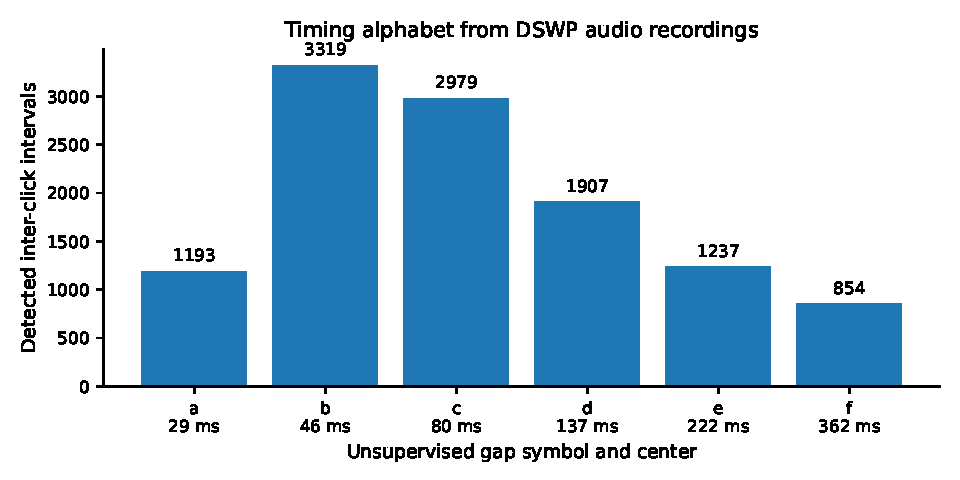
\includegraphics[width=0.82\linewidth]{fig1_timing_alphabet.pdf}
\caption{Unsupervised ICI timing alphabet estimated from DSWP audio recordings. Counts refer to detected inter-click intervals in accepted recordings.}
\label{fig:timing_alphabet}
\end{figure}

\begin{table}[H]
\centering
\caption{Timing alphabet from DSWP audio recordings. The model was fitted to log-ICI values and sorted by center duration.}
\label{tab:timing_alphabet}
\begin{tabular}{lrrrr}
\toprule
Symbol & Center (ms) & Count & 10th percentile (ms) & 90th percentile (ms) \\
\midrule
a & 29.3 & 1193 & 25.5 & 32.9 \\
b & 45.8 & 3319 & 37.3 & 55.9 \\
c & 79.5 & 2979 & 63.6 & 101.7 \\
d & 136.7 & 1907 & 113.7 & 172.0 \\
e & 222.0 & 1237 & 189.3 & 285.0 \\
f & 361.6 & 854 & 317.1 & 583.2 \\
\bottomrule
\end{tabular}
\end{table}

\subsection{Dense audio recordings are structured, not random}

The DSWP audio recordings separate into click-density families (Table~\ref{tab:audio_families}; Figure~\ref{fig:audio_density}). Sparse recordings have a median of 4 detected clicks and long mean ICIs; dense recordings have a median of 21 detected clicks and a median mean ICI of 75 ms. The shift is not merely additive. As density increases, the front-two mass decreases and fast timing symbols become more common, indicating a different mode of temporal organization.

\begin{figure}[H]
\centering
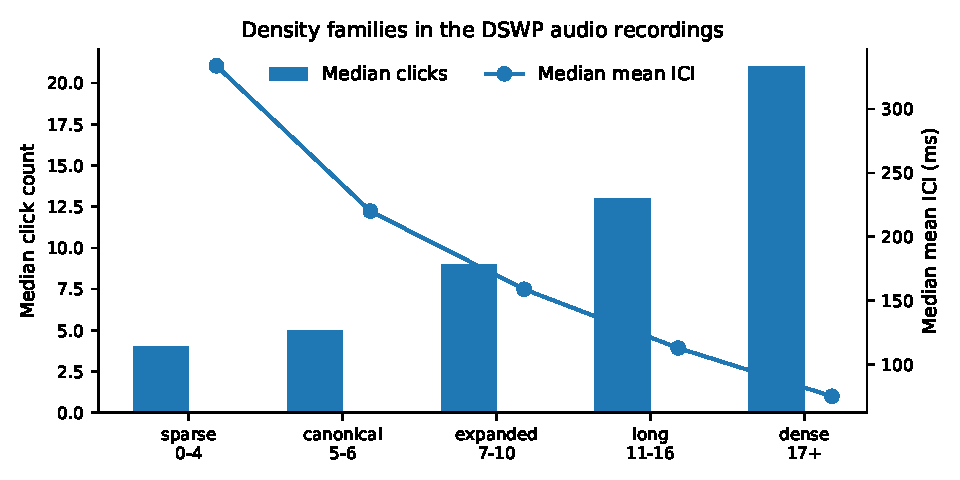
\includegraphics[width=0.82\linewidth]{fig2_audio_density_families.pdf}
\caption{Density families in DSWP audio recordings. Click count and mean ICI change systematically across sparse, canonical, expanded, long, and dense forms.}
\label{fig:audio_density}
\end{figure}

\begin{table}[H]
\centering
\caption{Audio density-family statistics from DSWP recordings.}
\label{tab:audio_families}
\small
\begin{tabular}{lrrrrr}
\toprule
Density family & $n$ & Median clicks & Median mean ICI (s) & Front-two mass & Fast share \\
\midrule
long 11--16 & 302 & 13 & 0.113 & 0.166 & 0.357 \\
expanded 7--10 & 273 & 9 & 0.159 & 0.275 & 0.167 \\
dense 17+ & 228 & 21 & 0.075 & 0.085 & 0.519 \\
canonical 5--6 & 163 & 5 & 0.220 & 0.571 & 0.000 \\
sparse 0--4 & 75 & 4 & 0.334 & 0.960 & 0.000 \\
\bottomrule
\end{tabular}
\end{table}

Motif-compression analysis further supports structure. Dense recordings had median top-12 bigram coverage of 0.813, compared with 0.500 for canonical 5--6 click forms and 0.000 for sparse forms (Table~\ref{tab:motif}). Thus dense trains are not arbitrary long tails of clicks; they are highly compressible sequences built from recurring timing motifs.

\begin{table}[H]
\centering
\caption{Motif compression by audio density family. Coverage is the fraction of adjacent timing-symbol bigrams belonging to the twelve most frequent bigrams in the audio corpus.}
\label{tab:motif}
\begin{tabular}{lrrr}
\toprule
Density family & Strings analyzed & Median coverage & Mean coverage \\
\midrule
canonical 5--6 & 163 & 0.500 & 0.478 \\
dense 17+ & 228 & 0.813 & 0.784 \\
expanded 7--10 & 273 & 0.429 & 0.456 \\
long 11--16 & 302 & 0.556 & 0.567 \\
sparse 0--4 & 74 & 0.000 & 0.169 \\
\bottomrule
\end{tabular}
\end{table}

\subsection{R2 behaves as a carrier frame in the annotated dialogue table}

In the annotated dialogue table, R2 accounts for 2,359 of 3,840 events (61.4\%). It has median click count 5 and a median duration of 1.142 s. R2 is enriched in medial bout position and depleted at bout boundaries: its start lift is 0.742 and end lift is 0.821. This is the central empirical reason for treating R2 as a carrier frame. It appears to maintain an ongoing exchange rather than preferentially opening or closing one.

\begin{table}[H]
\centering
\caption{Selected rhythm-class operator profiles from the annotated dialogue table. $R$ is the release rhythm index. Switch and overlap are computed for same-REC adjacent rows only.}
\label{tab:operator_profiles}
\begin{tabular}{lrrrrrr}
\toprule
Class & Count & Share & Start lift & End lift & Switch next & Overlap next \\
\midrule
R2 & 2359 & 0.614 & 0.742 & 0.821 & 0.632 & 0.280 \\
R4 & 561 & 0.146 & 1.151 & 1.151 & 0.590 & 0.166 \\
R0 & 272 & 0.071 & 0.691 & 0.820 & 0.722 & 0.338 \\
R17 & 175 & 0.046 & 1.409 & 0.671 & 0.577 & 0.256 \\
R16 & 94 & 0.024 & 1.749 & 1.249 & 0.589 & 0.200 \\
R13 & 57 & 0.015 & 2.472 & 2.060 & 0.313 & 0.042 \\
R7 & 54 & 0.014 & 3.262 & 2.827 & 0.689 & 0.200 \\
R11 & 43 & 0.011 & 3.004 & 2.185 & 0.333 & 0.083 \\
R15 & 29 & 0.008 & 2.430 & 2.025 & 0.407 & 0.037 \\
R14 & 13 & 0.003 & 1.807 & 3.613 & 0.167 & 0.000 \\
\bottomrule
\end{tabular}
\end{table}

\begin{figure}[H]
\centering
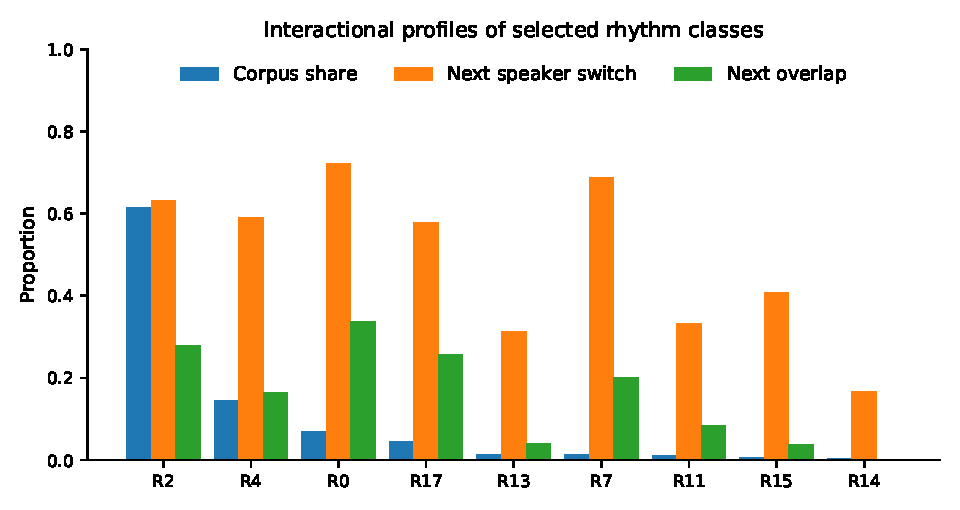
\includegraphics[width=0.82\linewidth]{fig3_operator_rates.pdf}
\caption{Corpus share, speaker-switch rate, and overlap rate for selected rhythm classes. R0 has a high switch and overlap profile despite low corpus share. R13, R11, R15, and R14 are boundary-enriched classes with lower switch profiles.}
\label{fig:operator_rates}
\end{figure}

\subsection{R0 and R17 form high-engagement transition patterns}

Pair statistics reveal stronger operator structure than single-class frequencies alone. R0--R2 and R2--R0 pairs are overwhelmingly cross-whale. R0 $\rightarrow$ R2 has a cross-whale rate of 0.910 and an overlap rate of 0.448. R2 $\rightarrow$ R0 has a cross-whale rate of 0.930 and an overlap rate of 0.434. This motivates the gloss of R0 as a handoff, entry, or addressive operator in the R2 carrier frame.

R17 behaves differently. It is a dense class, with median click count 18 and median mean ICI 60 ms. The pair R17 $\rightarrow$ R0 has a cross-whale rate of 0.958, an overlap rate of 0.583, and a median gap of -0.546 s. The negative median gap means that R0 often begins before the dense R17 signal has finished. R17 is therefore not well described as a merely long coda; it is a candidate escalation or co-vocal transition operator.

\begin{table}[H]
\centering
\caption{Selected adjacent-pair statistics. Pair rows are included only when $n \geq 10$. Gap is next onset minus current offset; negative values indicate overlap.}
\label{tab:pair_stats}
\begin{tabular}{lrrrr}
\toprule
Pair & $n$ & Cross-whale rate & Overlap rate & Median gap (s) \\
\midrule
R2 $\rightarrow$ R2 & 1753 & 0.583 & 0.257 & 2.471 \\
R0 $\rightarrow$ R2 & 134 & 0.910 & 0.448 & 0.211 \\
R2 $\rightarrow$ R0 & 129 & 0.930 & 0.434 & 0.555 \\
R17 $\rightarrow$ R2 & 60 & 0.800 & 0.317 & 1.785 \\
R2 $\rightarrow$ R17 & 59 & 0.898 & 0.373 & 0.678 \\
R17 $\rightarrow$ R17 & 52 & 0.135 & 0.058 & 2.099 \\
R0 $\rightarrow$ R17 & 26 & 1.000 & 0.423 & 0.993 \\
R17 $\rightarrow$ R0 & 24 & 0.958 & 0.583 & -0.546 \\
R13 $\rightarrow$ R13 & 16 & 0.063 & 0.063 & 4.727 \\
\bottomrule
\end{tabular}
\end{table}

\begin{figure}[H]
\centering
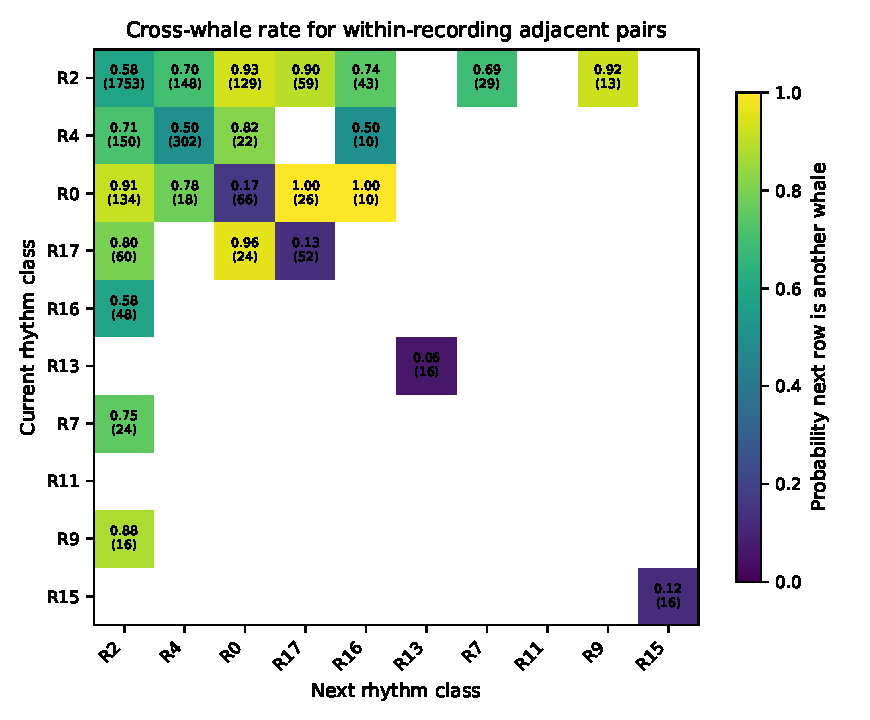
\includegraphics[width=0.78\linewidth]{fig5_pair_heatmap.pdf}
\caption{Cross-whale rate for selected same-REC adjacent rhythm pairs. Numbers in cells show rate and count. High R0--R2 and R17--R0 rates motivate handoff and escalation glosses.}
\label{fig:pair_heatmap}
\end{figure}

\subsection{Boundary-enriched classes suggest closure and transition operators}

R13, R11, R15, and R14 are enriched at bout boundaries and have lower switch or overlap rates than R0. R14 has end lift 3.613 and switch rate 0.167; R13 has start lift 2.472, end lift 2.060, and median next gap 4.51 s; R11 has start lift 3.004 and switch rate 0.333. These profiles support boundary or closure glosses. R7 is boundary-enriched but has a high switch rate (0.689), so it is better treated as a marked transition or opener candidate than as a simple closure form.

\subsection{Microtiming inside R2 changes interactional outcome}

R2 is common enough to test internal timing variation. In the slowest duration quartile of R2 codas, the high-front-mass half shows a speaker-switch rate of 0.571, compared with 0.384 for the low-front-mass half. Overlap also rises from 0.231 to 0.340 (Table~\ref{tab:r2_micro}; Figure~\ref{fig:r2_micro}). The two subsets have similar median durations (1.321 s vs. 1.342 s). The difference is therefore not simply that one group is longer. It is a difference in internal geometry within the same rhythm class and duration region.

\begin{table}[H]
\centering
\caption{R2 slow-quartile microtiming minimal pair. Front-two mass is $p_1+p_2$, the fraction of normalized duration occupied by the first two ICIs.}
\label{tab:r2_micro}
\begin{tabular}{lrrrrr}
\toprule
R2 subset & $n$ & Switch & Overlap & Median duration (s) & Median front-two mass \\
\midrule
Low front mass & 281 & 0.384 & 0.231 & 1.342 & 0.672 \\
High front mass & 282 & 0.571 & 0.340 & 1.321 & 0.692 \\
\bottomrule
\end{tabular}
\end{table}

\begin{figure}[H]
\centering
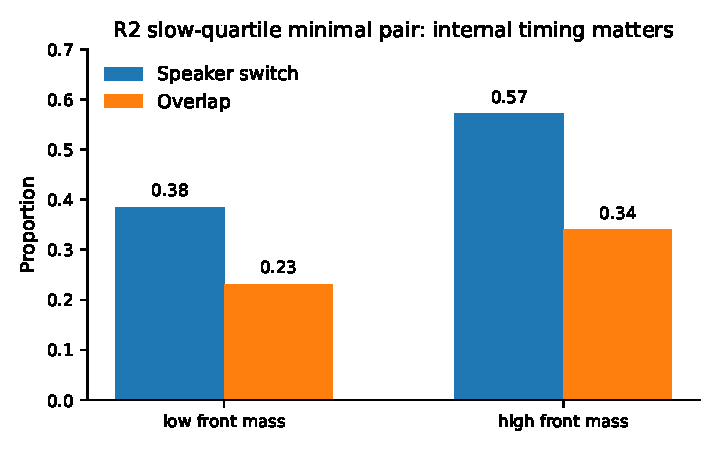
\includegraphics[width=0.62\linewidth]{fig4_r2_microtiming.pdf}
\caption{Within-class minimal pair for slow R2 codas. A modest increase in front-loading is associated with a large increase in next-speaker switching and overlap.}
\label{fig:r2_micro}
\end{figure}

\subsection{Fine timing predicts interactional outcomes better than rhythm class alone}

Grouped cross-validation shows that rhythm class alone is a weak predictor of whether the next coda comes from another whale. $R$-only AUC is 0.527. Adding duration and density raises AUC to 0.589. Fine timing without $R$ reaches 0.607, and full timing plus $R$ reaches 0.612 (Table~\ref{tab:auc}; Figure~\ref{fig:auc}). These are not high enough for a translation system. They are high enough to reject the view that the release rhythm label is the only interactionally relevant timing feature.

\begin{table}[H]
\centering
\caption{Grouped five-fold AUC for predicting whether the next same-REC coda is produced by a different annotated speaker. Folds are grouped by REC.}
\label{tab:auc}
\begin{tabular}{lrr}
\toprule
Feature set & Mean AUC & SD across folds \\
\midrule
$R$ only & 0.527 & 0.024 \\
$R$ + duration/density & 0.589 & 0.044 \\
Timing without $R$ & 0.607 & 0.050 \\
Full timing + $R$ & 0.612 & 0.044 \\
\bottomrule
\end{tabular}
\end{table}

\begin{figure}[H]
\centering
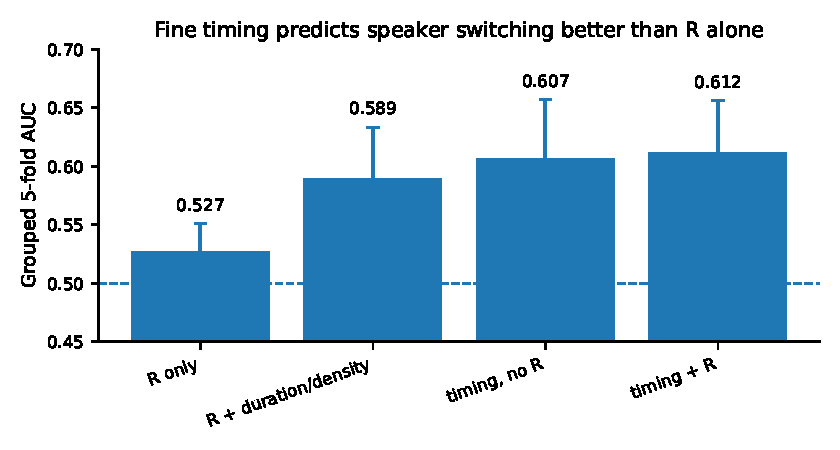
\includegraphics[width=0.72\linewidth]{fig6_auc.pdf}
\caption{AUC comparison for next-speaker switch prediction. Fine timing features outperform the rhythm index alone under grouped cross-validation by recording identifier.}
\label{fig:auc}
\end{figure}

\section{Empirical interpretation: a temporal-operator lexicon}

Table~\ref{tab:functional_lexicon} gives a functional lexicon justified by the preceding statistics. These glosses are not literal translations. They are hypotheses about interactional force.

\begin{table}[H]
\centering
\caption{Provisional temporal-operator lexicon. Glosses summarize statistical behavior, not literal semantic content.}
\label{tab:functional_lexicon}
\begin{tabular}{P{0.15\linewidth}P{0.33\linewidth}P{0.41\linewidth}}
\toprule
Form & Candidate functional gloss & Evidence \\
\midrule
R2 & Carrier frame; maintenance of ongoing exchange & Dominates corpus (61.4\%); depleted at bout boundaries; often returns after inserted forms \\
\addlinespace
R0 & Handoff, entry, or addressive slot-opening operator & High switch (0.722), high overlap (0.338), strong R0--R2 cross-whale pairings \\
\addlinespace
R17 & Dense escalation or co-vocal transition operator & Median 18 clicks; fast mean ICI; R17 $\rightarrow$ R0 has high overlap and negative median gap \\
\addlinespace
R13, R11, R15, R14 & Boundary, settling, or closure candidates & Boundary lift greater than 2 for several classes; lower switch and longer gaps \\
\addlinespace
High-front-mass R2 & More addressive or response-eliciting variant of carrier & Same rhythm and slow duration region, but switch rises from 0.384 to 0.571 \\
\addlinespace
Dense audio timing strings & Intensified shared-clock mode or train mode & High click count, short ICIs, high top-12 bigram coverage \\
\bottomrule
\end{tabular}
\end{table}

The central claim is that the communication layer recoverable from the available public data is operational rather than referential. R2 can be common without being trivial, because carrier frames in interactional systems are expected to be common. R0 can be rare but high-force, because handoff or addressive markers need not dominate the corpus. R17 can be dense and overlap-heavy because escalation or co-vocal entry may involve occupying the acoustic channel rather than politely waiting for a turn boundary.

\section{Discussion}

\subsection{Why a pure contact-call interpretation is insufficient}

A generic contact-call interpretation cannot explain the observed asymmetries. If the main function of all common forms were simply presence marking, then R0, R2, and R17 would be expected to have similar switch and overlap profiles after conditioning on frequency. They do not. R2 is frequent and medial. R0 is less frequent but high-switch and high-overlap. R17 is dense and participates in overlapping transition pairs. Boundary-enriched classes show low-switch, long-gap behavior. These differences are interactional, not merely distributional.

\subsection{Why rhythm labels are insufficient}

The AUC analysis and R2 minimal pair both show that $R$ is an incomplete representation. $R$ captures a useful normalized shape, but continuous timing geometry changes the likely next state of the exchange. This supports the Project CETI view that coda structure is combinatorial and context-sensitive, and extends it by interpreting some of the variation as operator force.

\subsection{Relation to spectral-vowel work}

The present analysis is intentionally timing-centered. Spectral-vowel work suggests that additional dimensions may combine with timing features \citep{begus2025vowels,begus2026phonology}. If spectral classes can be assigned to the same annotated timelines, the operator model predicts interactions: a given timing operator may have different force depending on spectral quality, just as human syllables can combine segmental and prosodic features.

\subsection{Relation to automatic detection and WhAM}

Automatic coda detection and generative acoustic modeling address complementary problems. A detector supplies larger and cleaner event tables; a generative model supplies embeddings and counterfactual synthesis. The operator framework supplies an evaluation target: embeddings should not only classify coda types, but also predict future interactional state. A strong model should preserve R0-like handoff effects, R17-like overlap effects, and R2 microtiming effects under held-out recording evaluation.

\section{Limitations and non-claims}

Several limits are essential.

\begin{enumerate}
    \item The DSWP audio recordings are not aligned to rows of \path{sperm-whale-dialogues.csv}. No audio-level result is used to claim that a particular recording caused a particular response.
    \item Speaker IDs are available in the annotated dialogue table but not in the DSWP audio recordings. All speaker-switch statistics come from the annotated table.
    \item The operator glosses are observational. Without behavior, localization, depth, distance, age/sex class, and recipient information, causal semantic translation is not established.
    \item The click detector for the audio corpus is transparent but simple. A stronger detector may change exact counts and timing-symbol frequencies, though the broad density-family result should be testable.
    \item AUC values are modest. They support the claim that timing contains interactional information; they do not support a standalone decoder.
\end{enumerate}

\section{Reproducibility}

The supplementary package contains the LaTeX source, figures, data tables, and scripts. Running
\begin{lstlisting}
python scripts/reproduce_statistics.py
python scripts/make_figures.py
latexmk -pdf main.tex
\end{lstlisting}
from the package root recomputes the tables and figures from the included tabular artifacts. To regenerate the DSWP audio feature table from a local copy of the Hugging Face audio files, run
\begin{lstlisting}
python scripts/extract_audio_recording_features.py /path/to/DSWP --out data/dswp_audio_recording_features.csv
\end{lstlisting}
The exact numerical values in this manuscript are those in the included tables under \texttt{tables/}. The raw public sources are \path{pratyushasharma/sw-combinatoriality} for the annotated timing artifacts and \path{orrp/DSWP} for the DSWP audio recordings.

\section{Conclusion}

The available public data support a richer interpretation of sperm whale coda structure than a flat coda-type inventory. DSWP audio recordings show a structured timing alphabet and dense motif-compressed train forms. The annotated dialogue corpus shows that rhythm classes have distinct interactional profiles: R2 behaves like a carrier frame, R0 like a handoff or entry operator, R17 like an escalation or co-vocal transition operator, and several rarer classes like boundary or closure operators. Fine timing within R2 changes next-speaker outcomes, and timing features outperform rhythm class alone in grouped prediction.

The result is not a whale-to-English dictionary. It is a reproducible first-layer translation into functional operator language. The next step is to add behavioral and spatial context, spectral-vowel labels, and stronger audio-source separation so that operator glosses can be tested against changes in movement, distance, group composition, and activity state.

\appendix

\section{Appendix A: variable dictionary}

\begin{longtable}{P{0.16\linewidth}P{0.75\linewidth}}
\caption{Notation and variables.}\label{tab:variables}\\
\toprule
Symbol or field & Definition \\
\midrule
\endfirsthead
\toprule
Symbol or field & Definition \\
\midrule
\endhead
$n_i$ & Number of detected or annotated clicks in coda $i$. \\
$d_i$ & Duration of coda $i$, equal to \path{Duration} in the annotated dialogue table. \\
$\Delta_{i,j}$ & Inter-click interval $j$ of coda $i$, from ICI columns or from audio click detection. \\
$p_i$ & Normalized ICI vector $\Delta_i/\sum_j\Delta_{i,j}$. \\
$c_i$ & Normalized cumulative click-position vector beginning at 0 and ending at 1. \\
$R_i$ & Rhythm-template index from \path{rhythms.p}; an integer from 0 to 17. \\
$T_i$ & Tempo/duration-band index from \path{tempos-dict.p}; used descriptively, not as a complete per-row predictor. \\
$O_i$ & Ornament flag from \path{ornaments.p}. \\
\path{REC} & Recording or timeline identifier in \path{sperm-whale-dialogues.csv}. \\
\path{Whale} & Annotated speaker identity in \path{sperm-whale-dialogues.csv}. \\
$t_i$ & Coda onset time, \path{TsTo}. \\
$e_i$ & Coda end time, $t_i+d_i$. \\
$g_i$ & Next gap, $t_{i+1}-e_i$. Negative values indicate temporal overlap. \\
$S_i$ & Speaker-switch indicator for adjacent same-\path{REC} pairs. \\
$V_i$ & Overlap indicator for adjacent same-\path{REC} pairs. \\
Front-two mass & $p_{i,1}+p_{i,2}$, the normalized duration occupied by the first two ICIs. \\
Gap string & DSWP audio ICI sequence after quantization into symbols $a$--$f$. \\
Density family & Audio class by detected click count: sparse, canonical, expanded, long, dense. \\
\bottomrule
\end{longtable}

\section{Appendix B: tempo bands}

\begin{table}[H]
\centering
\caption{Recovered tempo-duration bands from the tempo dictionary. $T5$ was empty in this artifact and is omitted. Values summarize durations contained in the tempo dictionary, not necessarily all rows after exact matching.}
\label{tab:tempo_bands}
\begin{tabular}{lrrrrrr}
\toprule
Tempo & $n$ & Min (s) & P25 (s) & Median (s) & P75 (s) & Max (s) \\
\midrule
T0 & 723 & 0.000 & 0.310 & 0.322 & 0.334 & 0.391 \\
T1 & 236 & 0.393 & 0.458 & 0.490 & 0.511 & 0.591 \\
T2 & 743 & 0.597 & 0.738 & 0.785 & 0.834 & 0.907 \\
T3 & 524 & 0.907 & 0.970 & 1.002 & 1.044 & 1.090 \\
T4 & 1582 & 1.091 & 1.193 & 1.268 & 1.340 & 3.453 \\
\bottomrule
\end{tabular}
\end{table}

\section{Appendix C: figure and value provenance}

\begin{longtable}{P{0.18\linewidth}P{0.36\linewidth}P{0.36\linewidth}}
\caption{Source table for each main result.}\label{tab:provenance}\\[-0.6em]
\footnotesize\\
\toprule
Result & Data source & Reproduction file \\
\midrule
\endfirsthead
\toprule
Result & Data source & Reproduction file \\
\midrule
\endhead
Figure~\ref{fig:timing_alphabet}, Table~\ref{tab:timing_alphabet} & DSWP audio recordings after click detection; ICI mixture model & \path{data/dswp_audio_timing_alphabet.csv}; \path{scripts/extract_audio_recording_features.py}; \path{scripts/make_figures.py} \\
Figure~\ref{fig:audio_density}, Table~\ref{tab:audio_families} & DSWP audio feature table; density class by click count & \path{data/dswp_audio_recording_features.csv}; \path{tables/dswp_audio_density_family_stats.csv} \\
Table~\ref{tab:motif} & DSWP audio timing-symbol strings; top-12 bigram coverage & \path{tables/dswp_audio_motif_compression.csv} \\
Table~\ref{tab:operator_profiles}, Figure~\ref{fig:operator_rates} & \path{sperm-whale-dialogues.csv}, \path{rhythms.p}, \path{ornaments.p}; same-\path{REC} adjacency & \path{tables/dialogue_operator_stats.csv} \\
Table~\ref{tab:pair_stats}, Figure~\ref{fig:pair_heatmap} & Same annotated dialogue sources; adjacent rhythm pairs with $n \geq 10$ & \path{tables/dialogue_pair_stats.csv} \\
Table~\ref{tab:r2_micro}, Figure~\ref{fig:r2_micro} & Same annotated dialogue sources; R2 slowest duration quartile and front-two mass split & \path{tables/r2_slowest_frontloading_minimal_pair.csv} \\
Table~\ref{tab:auc}, Figure~\ref{fig:auc} & Same annotated dialogue sources; grouped logistic-regression cross-validation by \path{REC} & \path{tables/switch_prediction_auc_grouped.csv}; \path{tables/switch_prediction_auc_folds.csv} \\
\bottomrule
\end{longtable}

\section{Appendix D: complete reproduction commands}

The package is organized as follows:
\begin{lstlisting}
main.tex
references.bib
figures/
tables/
data/
scripts/
\end{lstlisting}

A clean reproduction from the included tabular artifacts is:
\begin{lstlisting}
python scripts/reproduce_statistics.py
python scripts/make_figures.py
latexmk -pdf main.tex
\end{lstlisting}

A raw-audio reproduction requires downloading \path{orrp/DSWP} and running the transparent click detector:
\begin{lstlisting}
python scripts/extract_audio_recording_features.py /path/to/DSWP \
    --out data/dswp_audio_recording_features.csv
\end{lstlisting}
Then rerun the statistics and figure scripts. Differences from the printed values may arise if a different DSWP snapshot, audio decoder, or peak detector threshold is used. The annotated-dialogue values should be exactly reproducible from the included \path{sperm-whale-dialogues.csv}, \path{rhythms.p}, and \path{ornaments.p} files.


\begin{thebibliography}{99}

\bibitem[Sharma et~al.(2024)]{sharma2024contextual}
Sharma, P., Gero, S., Payne, R., Gruber, D.~F., Rus, D., Torralba, A., and Andreas, J. (2024).
\newblock Contextual and combinatorial structure in sperm whale vocalisations.
\newblock \emph{Nature Communications}, 15:3617. doi:10.1038/s41467-024-47221-8.

\bibitem[Sharma(2024)]{swcombinatoriality}
Sharma, P. (2024).
\newblock \path{pratyushasharma/sw-combinatoriality}: dataset and codebase for contextual and combinatorial structure in sperm whale vocalisations.
\newblock Zenodo release. doi:10.5281/zenodo.10817697.

\bibitem[Paradise et~al.(2025a)]{dswpdataset}
Paradise, O. and collaborators (2025a).
\newblock Dominica Sperm Whale Project (DSWP) dataset.
\newblock Hugging Face dataset card: \path{orrp/DSWP}.

\bibitem[Paradise et~al.(2025b)]{paradise2025wham}
Paradise, O., Muralikrishnan, P., Chen, L., Flores Garcia, H., Pardo, B., Diamant, R., Gruber, D.~F., Gero, S., and Goldwasser, S. (2025b).
\newblock WhAM: Towards a translative model of sperm whale vocalization.
\newblock \emph{Advances in Neural Information Processing Systems}; arXiv:2512.02206.

\bibitem[Gubnitsky et~al.(2025)]{gubnitsky2025automatic}
Gubnitsky, G., Mevorach, Y., Gero, S., Gruber, D.~F., and Diamant, R. (2025).
\newblock Automatic detection and annotation of eastern Caribbean sperm whale codas.
\newblock \emph{Scientific Reports}, 15:12790. doi:10.1038/s41598-025-97009-z.

\bibitem[Begus et~al.(2025)]{begus2025vowels}
Begus, G., Sprouse, R.~L., Leban, A., Silva, M., and Gero, S. (2025).
\newblock Vowel- and diphthong-like spectral patterns in sperm whale codas.
\newblock \emph{Open Mind}, 9:1849--1874. doi:10.1162/OPMI.a.252.

\bibitem[Begus et~al.(2026)]{begus2026phonology}
Begus, G. and collaborators (2026).
\newblock The phonology of sperm whale coda vowels.
\newblock \emph{Proceedings of the Royal Society B}, 293(2069):20252994.

\bibitem[Hersh et~al.(2026)]{hersh2026mediterranean}
Hersh, T.~A., Alexiadou, P., Brotons, J.~M., Cerda, M., Pirotta, E., Frantzis, A., and Rendell, L. (2026).
\newblock Dialect variation in Mediterranean sperm whales shows evidence of cultural evolution in an isolated population.
\newblock \emph{Proceedings of the Royal Society B}, 293(2073):20260165. doi:10.1098/rspb.2026.0165.

\bibitem[Gero et~al.(2016)]{gero2016identity}
Gero, S., Whitehead, H., and Rendell, L. (2016).
\newblock Individual, unit and vocal clan level identity cues in sperm whale codas.
\newblock \emph{Royal Society Open Science}, 3(1):150372. doi:10.1098/rsos.150372.

\bibitem[Rendell and Whitehead(2003)]{rendell2003clans}
Rendell, L.~E. and Whitehead, H. (2003).
\newblock Vocal clans in sperm whales (\emph{Physeter macrocephalus}).
\newblock \emph{Proceedings of the Royal Society of London. Series B: Biological Sciences}, 270(1512):225--231. doi:10.1098/rspb.2002.2239.

\bibitem[Schulz et~al.(2008)]{schulz2008overlapping}
Schulz, T.~M., Whitehead, H., Gero, S., and Rendell, L. (2008).
\newblock Overlapping and matching of codas in vocal interactions between sperm whales: insights into communication function.
\newblock \emph{Animal Behaviour}, 76(6):1977--1988. doi:10.1016/j.anbehav.2008.07.032.

\bibitem[Whitehead(2003)]{whitehead2003sperm}
Whitehead, H. (2003).
\newblock \emph{Sperm Whales: Social Evolution in the Ocean}.
\newblock University of Chicago Press.

\end{thebibliography}

\end{document}
